\documentclass[usenames,dvipsnames]{article}

\usepackage{amsthm}
\usepackage{amsmath}
\usepackage{multicol}
\usepackage{amssymb}
\usepackage{mathabx}
\usepackage{accents}
\usepackage[english]{babel}
\usepackage{blindtext}
\usepackage{graphicx}
\usepackage{multicol}

\usepackage{tikz}
\usepackage{tkz-berge}
\usepackage{tkz-graph}

\usetikzlibrary{patterns,arrows,decorations.pathreplacing}

\usepackage{xcolor}
\definecolor{dblue}{RGB}{20,66,129}
\definecolor{rose}{RGB}{255,101,122}
\definecolor{crimsonred}{RGB}{132,22,23}
\definecolor{darkblue}{RGB}{72,61,139}

\definecolor{deepblue}{RGB}{36,123,160}
\definecolor{deepred}{RGB}{255,22,84}
\definecolor{deeporange}{RGB}{240,111,62}

\definecolor{olive}{rgb}{0.3, 0.4, .1}
\definecolor{fore}{RGB}{249,242,215}
\definecolor{back}{RGB}{51,51,51}
\definecolor{title}{RGB}{255,0,90}
\definecolor{dgreen}{rgb}{0.,0.6,0.}
\definecolor{gold}{rgb}{1.,0.84,0.}
\definecolor{JungleGreen}{cmyk}{0.99,0,0.52,0}
\definecolor{BlueGreen}{cmyk}{0.85,0,0.33,0}
\definecolor{RawSienna}{cmyk}{0,0.72,1,0.45}
\definecolor{Magenta}{cmyk}{0,1,0,0}





\theoremstyle{plain}
\newtheorem{lemma}{Lemma}
\newtheorem{prop}{Proposition}
\newtheorem*{example}{Example}
\newtheorem*{fact}{Fact}
\newtheorem{corollary}{Corollary}

\usepackage{algorithm}
\usepackage[noend]{algpseudocode}

\theoremstyle{plain}
\newtheorem{theorem}{Theorem}
\newtheorem{proposition}[theorem]{Proposition}
\newtheorem*{remark}{Remark}

\def\changemargin#1#2{\list{}{\rightmargin#2\leftmargin#1}\item[]}
\let\endchangemargin=\endlist 

\DeclareMathOperator{\codim}{codim}
\DeclareMathOperator{\lhdim}{\underline{\dim}_{\mathbf{M}}}
\DeclareMathOperator{\lmbdim}{\underline{\dim}_{\mathbf{MB}}}
\DeclareMathOperator{\biggercup}{\mathbin{\bigcup}}%

\title{Cartesian Products Avoiding Patterns}

\author{Jacob Denson\\ \and Malabika Pramanik\\ \and Joshua Zahl}

\begin{document}

\maketitle

\begin{abstract}
	We construct subsets of $[0,1]^d$ with large Hausdorff dimension whose Cartesian product avoids a set with low Minkowski dimension. This generalizes the pattern avoidance problem found in the literature. Given $Z \subset (\mathbf{R}^d)^n$ covered by the countable union of compact sets with lower Minkowski dimension at most $\alpha$, we construct a Cantor type set $X$ with Hausdorff dimension $(nd - \alpha) / (n-1)$ such that for any distinct $x_1, \dots, x_n \in X$, $(x_1, \dots, x_n) \not \in Z$.
	%
		In particular, our result generalizes Fraser and Pramanik's result on pattern avoidance, which assume $Z$ is smooth.
	%TODO FIX THIS SENTENCE
	%
	We use the result to construct high dimensional sets whose sum set avoids a given set, as well as construct subsets avoiding isoceles triangles. General pattern avoidance methods in the literature can only construct subsets of Euclidean space avoiding configurations, which makes the latter result particularly surprising.
\end{abstract}

% Ergodic Theoretic Connections: Furstenberg Katznelson and Weiss. Ziegler sets of positive density.

Can subsets of $\mathbf{R}^d$ with large fractional dimension be constructed avoiding patterns? For instance, is it possible to find a high dimensional set containing no colinear triple of points, or not containing any three points forming an isosceles triangle? If the pattern is specified as the zero set of a smooth function $f: (\mathbf{R}^d)^n \to \mathbf{R}$, then results in \cite{MalabikaRob} and \cite{Mathe} give general methods for finding $X$ such that for any distinct points $x_1, \dots, x_n \in X$, $f(x_1, \dots, x_n) = 0$. Rather than avoiding the zeroes of a function, in this paper, we fix a set $Z \subset (\mathbf{R}^d)^n$, and construct sets $X$ such that for any distinct $x_1, \dots, x_n \in X$, $(x_1, \dots, x_n) \not \in Z$. Surprisingly, in this setting we can obtain results only assuming conditions on the fractional dimension of $Z$.

\begin{theorem}
	Suppose $Z \subset (\mathbf{R}^d)^n$ is the countable union of compact sets with lower Minkowski dimension at most $\alpha$. Then there exists $X \subset [0,1]^d$ with
	%
	\[ \dim_{\mathbf{H}}(X) = \min \left( \frac{nd - \alpha}{n-1}, d \right), \]
	%
	such that if $x_1, \dots, x_n \in X$ are distinct, $(x_1, \dots, x_n) \not \in Z$.
\end{theorem}

% NOTE TO JOSH AND MALABIKA: DO WE STILL NEED TO EMPHASIZE THAT THE PATTERNS ARE DIFFICULT TO AVOID BECAUSE THEY ARE EVERYWHERE?

One advantage of the Cartesian product approach we have taken to the problem is that certain geometric features of $Z$ are more explicit than when $Z$ is expressed as the zero set of the function. In particular, studying the difficulty of the problem in terms of the fractional dimension of $Z$ is completely non-obvious from the functional perspective.

Despite the generality of our theorem, we are still able to recover Theorems 1.1 and 1.2 of \cite{MalabikaRob} as special cases when $Z$ is formed from a countable collection of smooth manifolds. Meanwhile, our proof is less technical than their result. Furthermore, our result shows that the results remains robust under small changes in the fractional dimension of $Z$. Section 6 is devoted to a comparison of our method with \cite{MalabikaRob}, as well as other generic pattern avoidance methods.

Because our result can be applied to very general sets $Z$, we can apply the result to yield a great many interesting pattern avoiding sets. In particular, we can find large subsets of Euclidean space whose sums avoid a given set. Most interesting of the applications is a `restricted' construction of a large set avoiding configurations, via use of a projection trick. In this scenario, in addition to a set $Z$, we are given an arbitrary set $Y$, and we must construct a high dimensional subset $X$ of $Y$ avoiding $Z$. None of the existing constructions are able to be applied to yield results of this form, because the patterns involved are highly irregular. The discussion of these applications is in Section 5.

The key idea to avoiding sparse configurations is a random mass equidistribution strategy. This is featured as the main technique in our solution to a discrete variant of the theorem in Section 2. This discrete problem is very difficult to solve optimally, but we use a random strategy which is optimal enough in expectation, and is likely tight for general inputs to the problem. By overlaying the solution to the discretized problem at a sequence of scales, in Section 3 we are able to obtain the required set $X$ via a Cantor-type construction.

An important property of our discrete strategy is that it provides an `equidistributed' mass selection strategy. Exploiting this, in Section 4 we are able to show the set $X$ has the required Hausdorff dimension regardless of how fast our sequence of scales decay. The equidistribution technique occurs implicitly in at least one other Hausdorff dimension calculation, for example, in \cite{MalabikaRob}. But we do not believe equidistribution has been explicitly identified in the literature as a method to maintain fractal dimension despite a rapid decay of scales used in the construction of the fractal.

\begin{remark}
	The difficult setting of Theorem 1 occurs when $\alpha \geq d$. If $\alpha < d$,
	%
	\[ X = \left\{ x \in [0,1]^d : x \neq z_k\ \text{for all}\ (z_1, \dots, z_n) \in Z\ \text{and $1 \leq k \leq d$} \right\} \]
	%
	gives a set with full Hausdorff dimension satisfying the properties of the theorem. In our proof, we will assume $d \leq \alpha < dn$, and so must find a set $X$ with Hausdorff dimension $(dn - \alpha) / (n - 1)$ avoiding the set $Z$.
\end{remark}

%\section{A Fractal Avoidance Framework}

%One way to think about generic pattern avoidance methods is to specify the pattern as the zero set of a function. For example,
%
%\begin{itemize}
%	\item A set $X \subset \mathbf{R}$ contains no three term arithmetic progressions if and only if for any distinct $x,y,z \in X$,
	%
%	\[ f(x,y,z) = x + z - 2y \neq 0  \]
	%
%	This function vanishes if and only if there exists $b$ and $t$ such that $x = b$, $y = b+t$, and $z = b+2t$.

%	\item A set $X \subset \mathbf{R}^d$ contains the vertices of no isosceles triangles if and only if for any three distinct $x,y,z \in X$,
	%
%	\[ f(x,y,z) = d(x,y) - d(y,z) \neq 0 \]
	%
%	If $f(x,y,z) = 0$, then the line segments $xy$ and $zy$ form the legs of the isoceles triangle.
	%The problem of avoiding this function is similar to the last example, since isosceles triangles are planar variants of three term arithmetic progressions.

%	\item A set $X \subset \mathbf{R}^d$ does not contain a family of angles $\{ \alpha \}$ if and only if for any distinct $x,y,z \in X$, and $\alpha$,
	%
%	\[ f(x,y,z) = \frac{(x - z) \cdot (y - z)}{|x - z||y - z|} \neq \cos(\alpha) \]
	%
%	where the cosine formula for the dot product is used.

%	\item A set $X \subset \mathbf{R}^d$ does not contain $d+1$ points in a lower dimensional hyperplane if and only if for any distinct $x_0, \dots, x_d \in X$,
	%
%	\[ f(x_0, \dots, x_d) = \det(x_1 - x_0, \dots, x_d - x_0) \neq 0 \]
	%
%	If $\det(x_1 - x_0, \dots, x_d - x_0) = 0$, the vectors $x_1 - x_0, \dots, x_d - x_0$ are not linearly independent, and thus span a plane of dimension smaller than $d$.
%\end{itemize}
%
%This method of description is summarized by a general framework.

%\begin{changemargin}{0.5em}{0em}
%{\bf The Configuration Avoidance Problem:} Given a function $f: (\mathbf{R}^d)^n \to \mathbf{R}$, find $X \subset \mathbf{R}^d$ such that for any {\it distinct} $x_1, \dots, x_n \in X$, $f(x_1, \dots, x_n) \neq 0$, with as high a Hausdorff dimension as possible.
%\end{changemargin}

%The functional framework is common in the literature. For instance, it is the viewpoint behind the methods of \cite{MalabikaRob} and \cite{Mathe}, who give results assuming various regularity conditions on the function $f$. Here, we take the perspective that $f$ gives extraneous information irrelevant to the problem at hand. It's real importance is suggesting geometric properties of the zero set $Z$. Once $Z$ is taken as the primary object to study, the configuration avoidance problem becomes equivalent to another framework. It is the viewpoint of this paper that this framework is more flexible to work with, and thinking in terms of this framework leads to new general avoidance methods.

%\begin{changemargin}{0.5em}{0em}
%	{\bf The Fractal Avoidance Problem:} Given $Z \subset (\mathbf{R}^d)^n$, find $X \subset \mathbf{R}^d$ such that if $x_1, \dots, x_n \in X$ are {\it distinct}, $(x_1, \dots, x_n) \not \in Z$, with as high a Hausdorff dimension as possible.
%\end{changemargin}

%As is suggested by the fact that only the Cartesian product of distinct values of $x_1, \dots, x_n \in X$ are required to avoid $Z$, the diagonal set $\Delta$ of points $(x_1, \dots, x_n) \in (\mathbf{R}^d)^n$ such that $x_i = x_j$ for some $i \neq j$ plays a crucial role in the problem. If a point in $\Delta$ has a neighbourhood not intersecting $Z$, then by placing $X^n$ in this neighbourhood we find a full dimensional solution to the fractal avoidance problem. So in order for the problem to be nontrivial, $Z$ must be dense in a neighbourhood of $\Delta$. The structure of $Z$ around $\Delta$ therefore plays a major part in finding solutions to the fractal avoidance problem.

%We are free to pick any subset of $X$ we want. Because Hausdorff dimension is a local property of the set, we can always assume $X$ lies in a bounded region of space. Once this region is fixed, only a bounded portion of $Z$ could ever intersect $X^n$, allowing us to use compactness arguments. This is necessary to our method, and because of this, we work with a local version of the fractal avoidance framework, to which the general fractal avoidance problem can always be reduced by fixing a region, and changing coordinates.

%\begin{changemargin}{0.5em}{0em}
%	{\bf The Local Fractal Avoidance Problem:} Given $Z \subset ([0,1]^d)^n$, find $X \subset [0,1]^d$ such that if $x_1, \dots, x_n \in X$ are {\it distinct}, $(x_1, \dots, x_n) \not \in Z$.
%\end{changemargin}

%Since we are the first to introduce the fractal avoidance problem, a natural goal is to solve the general problem with minimal assumptions on $Z$. Here the only restriction we place on $Z$ is it's fractal dimension. Here we use the {\it lower Minkowski dimension} of a compact set $E$, defined as
%
%\[ \lhdim(E) = \liminf_{L \to 0} \frac{\log |\mathcal{B}(E,L)|}{\log(1/L)} \]
%
%Thus there is $L_k \to 0$ with $|\mathcal{B}(E,L_k)| = (1/L_k)^{\lhdim(E) + o(1)}$

%\begin{theorem}
%	If $Z$ is the countable union of sets with lower Minkowski dimension upper bounded by $\alpha$, with $\alpha \geq d$, then there is $X$ solving the local fractal avoidance problem for $Z$ with
	%
%	\[ \dim_{\mathbf{H}}(X) = \frac{dn - \alpha}{n - 1} = \frac{\codim_{\mathbf{H}}(Z)}{n - 1} \]
	%
	%See section 2 for a precise definition of lower Minkowski dimension we use.
%	One can view $dn - \alpha$ as the fractal codimension of $Z$ in $(\mathbf{R}^d)^n$.
%\end{theorem}

%\begin{remark}
%	If $Z$ is the union of sets with dimension $\alpha < d$, the set obtained from $[0,1]^d$ by removing the projections of $Z$ onto each coordinate has full Hausdorff dimension and trivially solves the local fractal avoidance problem. Thus we need not consider these parameters in our theorem.
%\end{remark}

%The aim of the theorem is to explore a general method for solving configuration avoidance problems. For particular configurations, it is highly likely that additional geometric features can be exploited to obtain avoiding sets with a much larger Hausdorff dimension. But our goal is not to find tight results for particular configurations. Instead, we want to show how much a single geometric feature of the configuration, in this case a bound on the dimension of the set $Z$, can be exploited. Other general results focus on other geometric features of the problem. For instance, the method of \cite{Mathe} explores what happens when $Z$ is a low dimensional algebraic variety. As more and more methods are revealed which exploit various features of the problem, we will be able to obtain tight results for particular configurations with ease, by synthesizing various approaches which exploit the most important geometric features of the configuration.

\section{Frequently Used Notation and Terminology}

\begin{itemize}
	\item For a length $l$, $\mathcal{B}^d_l$ denotes the family of all half open cubes in $\mathbf{R}^d$ with sidelength $l$ and corners on the lattice $(l \cdot \mathbf{Z})^d$. That is,
	%
	\[ \mathcal{B}^d_l = \{ [a_1,a_1 + l) \times \dots \times [a_d, a_d + l) : a_i \in l \cdot \mathbf{Z} \}. \]
	%
	If $E \subset \mathbf{R}^d$, $\mathcal{B}^d_l(E)$ is the family of cubes in $\mathcal{B}^d_l$ intersecting $E$, i.e.
	%
	\[\mathcal{B}^d_l(E) = \{ I \in \mathcal{B}^d_l: I \cap E \neq \emptyset \}. \]
	%
	For instance, $\mathcal{B}^d_l(\mathbf{R}^d) = \mathcal{B}^d_l$.

	\item The {\it lower Minkowski dimension} of a compact set $E \subset \mathbf{R}^d$ is
	%
	\[ \lhdim(E) = \liminf_{l \to 0} \frac{\log( \#( \mathcal{B}^d_l(E) ) )}{\log(1/l)}. \]
	%
	Thus there is $l_k \to 0$ with $\# ( \mathcal{B}^d_{l_k}(E) ) = (1/l_k)^{\lhdim(E) + o(1)}$.

	\item A {\it Frostman measure} of dimension $\alpha$ is a compactly supported finite Borel measure $\mu$ on $\mathbf{R}^d$ such that for any ball $B_r(x)$ of radius $r$ centered at a point $x$, $\mu(B_r(x)) \lesssim r^\alpha$. The {\it Hausdorff dimension} of a set $X \subset \mathbf{R}^d$ is
	%
	\[ \dim_{\mathbf{H}}(X) = \sup \left\{ \alpha: \begin{array}{c} \text{There is an}\ \alpha\ \text{dimensional Frostman}\\
	\text{measure supported on $X$} \end{array} \right\} \]

	% TODO: Introduce Hausdorff dimension by Frostman's lemma.

%	\item The {\it lower modified box counting dimension} of a set $E$ is
	%
%	\[ \lmbdim(E) = \inf \left\{ \sup \left( \lhdim(E_i) \right): E = \bigcup E_i \right\} \]
	%
%	Thus $E$ is covered by countably many sets $U_k$ with with lower Minkowski dimension upper bounded by $\lmbdim(E)$.

	\item Adopting the terminology of \cite{KatzTao}, we say a collection of sets $U_1, U_2, \dots$ is a {\it strong cover} of some set $E$ if $E \subset \limsup U_k$, which means every element of $E$ is contained in infinitely many of the sets $U_k$.

	\item Given $I \in \mathcal{B}^{dn}_l$, we can decompose $I$ as $I_1 \times \dots \times I_n$ for unique cubes $I_1, \dots, I_n \in \mathcal{B}^d_l$. We say $I$ is {\it non diagonal} if the cubes $I_1, \dots, I_n$ are distinct.
	% TODO: Don't use Non diagonal - weakly diagonal?

	% TODO: Define a dyadic scale.
\end{itemize}

\section{Avoidance at Discrete Scales}

We avoid $Z$ by considering an infinite sequence of scales. At each scale, we solve a discretized version of the problem. Combining these solutions then solves the original problem. This section describes the discretized avoidance technique. This is the {\it core} part of our construction, and the Hausdorff dimension we achieve is a direct result of our success in the discrete setting.

Fix two dyadic scales $l > s$. In the discrete setting, $Z$ is replaced by a union of sidelength $s$ cubes, denoted $Z'$. Our goal is to take a set $E$, which is a union of sidelength $l$ cubes, and carve out a union of sidelength $s$ cubes $F$ such that $F^n$ is disjoint from the non-diagonal cubes of $Z'$.

In order to ensure the Hausdorff dimension calculations of $X$ go smoothly, it is crucial that the mass of $F$ is spread uniformly over $E$ in the discrete setting. We can achieve this by trying to include a equal portion of mass in each sidelength $r$ subcube of $E$, for some intermediary dyadic scale $r \in (s,l)$ with $l > r > s$. The next lemma shows that we can select a equal portion of mass from {\it almost} all of the sidelength $r$ cubes.
% TODO: Add bounds which make the theorem trivial.

\begin{figure}[h]
	\centering
    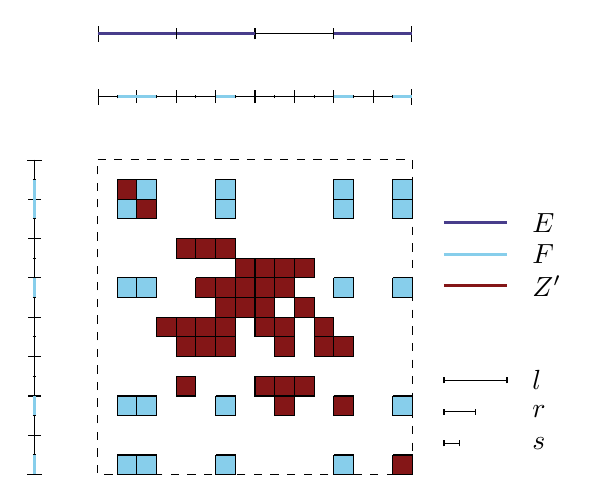
\begin{tikzpicture}[scale=4] %% Change scaling as needed
        \draw [|-]  (0,0) -- (1/4,0);
		\draw (0,0) -- (1,0);
        \draw [-|] (3/4,0) -- (1,0);% node [anchor = south west] {$E$};

        \foreach \x in {1,2,3}
        	\draw (\x/4,-0.5pt) -- (\x/4,0.5pt);

        \foreach \x in {0,1,3}
    		\draw[darkblue, very thick] (\x/4+0.001,0) -- (\x/4 + 1/4-0.001,0);




        \draw [|-]  (0,-0.2) -- (1/4,-0.2);
        \draw (0,-0.2) -- (1,-0.2);
        \draw [-|] (6/7,-0.2) -- (1,-0.2);% node [anchor = north west] {$F$};

        \foreach \x in {1,...,15}
            \draw (\x/16,-0.2-0.005) -- (\x/16,-0.2+0.005);

        \foreach \x in {1,...,7}
            \draw (\x/8,-0.2-0.02) -- (\x/8,-0.2+0.02);

        \foreach \x in {1,2,6,12,15}
            \draw[SkyBlue, very thick] (\x/16+0.001,-0.2) -- (\x/16 + 1/16 - 0.001,-0.2);








        \draw [|-]  (-0.2,-0.4) -- ++(0,-0.01);
        \draw (-0.2,-0.4) -- (-0.2,-1.4);
        \draw [-|] (-0.2,-1.38) -- (-0.2,-1.4);% node [anchor = north east] {$F$};

        \foreach \x in {1,...,15}
            \draw (-0.2-0.005,-0.4-\x/16) -- (-0.2+0.005,-0.4 -\x/16);

        \foreach \x in {1,...,7}
            \draw (-0.2-0.02,-0.4-\x/8) -- (-0.2+0.02,-0.4-\x/8);

        \foreach \x in {1,2,6,12,15}
        	\draw[SkyBlue, very thick] (-0.2,-0.4-\x/16-0.001) -- (-0.2,-0.4-\x/16-1/16+0.001);





        \draw[dashed] (0,-0.4) -- (1,-0.4) -- (1,-1.4) -- (0,-1.4) -- (0,-0.4);

        \foreach \x in {1,2,6,12,15}
        	\foreach \y in {1,2,6,12,15}
        		\draw[fill=SkyBlue] (\x/16,-0.4 - \y/16) -- ++(0,-1/16) -- ++ (1/16,0) -- ++(0,1/16) -- ++(-1/16,0);

        \foreach \x in {1,2,6,12,15}
        	\draw[fill=crimsonred] (\x/16,-0.4 - \x/16) -- ++(0,-1/16) -- ++ (1/16,0) -- ++(0,1/16) -- ++(-1/16,0);

        \foreach \x/\y in {4/4, 5/4, 6/4, 7/5, 8/5, 9/5, 10/5, 5/6, 6/6,7/6,8/6,9/6, 6/7, 7/7, 8/7, 10/7, 3/8, 4/8, 5/8, 6/8, 8/8, 9/8, 11/8, 4/9, 5/9, 6/9, 9/9, 11/9, 12/9, 4/11, 8/11, 9/11, 10/11, 9/12}
        	\draw[fill=crimsonred] (\x/16,-0.4 - \y/16) -- ++(0,-1/16) -- ++ (1/16,0) -- ++(0,1/16) -- ++(-1/16,0);







            \draw [darkblue, very thick] (1.1,-0.6) -- (1.3,-0.6);
%            \foreach \x in {1.1, 1.3}
%                \draw (\x,-0.6 - 0.01) -- (\x,-0.6 + 0.01);
            \draw (1.35,-0.6) node [anchor = west] {$E$};

            \draw [SkyBlue, very thick] (1.1,-0.7) -- (1.3,-0.7);
%            \foreach \x in {1.1,1.3}
%                \draw (\x,-0.7 - 0.01) -- (\x, -0.7 + 0.01);
            \draw (1.35,-0.7) node [anchor = west] {$F$};

            \draw [crimsonred, very thick] (1.1,-0.8) -- (1.3,-0.8);
%            \foreach \x in {1.1,1.3}
%                \draw (\x,-0.8 - 0.01) -- (\x, -0.8 + 0.01);
            \draw (1.35,-0.8) node [anchor = west] {$Z'$};

            \draw (1.1,-1.1) -- (1.3,-1.1);
            \foreach \x in {1.1, 1.3}
                \draw (\x,-1.1 - 0.01) -- (\x,-1.1 + 0.01);
            \draw (1.35,-1.1) node [anchor = west] {$l$};

            \draw (1.1,-1.2) -- (1.2,-1.2);
            \foreach \x in {1.1, 1.2}
                \draw (\x,-1.2 - 0.01) -- (\x,-1.2 + 0.01);
            \draw (1.35,-1.2) node [anchor = west] {$r$};

            \draw (1.1,-1.3) -- (1.15,-1.3);
            \foreach \x in {1.1, 1.15}
                \draw (\x,-1.3 - 0.01) -- (\x,-1.3 + 0.01);
            \draw (1.35,-1.3) node [anchor = west] {$s$};
	\end{tikzpicture}
	\caption{An example choice of $F$ in Lemma 1 where $d = 1$ and $n = 2$. $F$ satisfies the non-concentration and avoidance property, as well as containing an interval from all but 3 of the intervals in $\mathcal{B}^d_r(E)$.}
\end{figure}
%TODO: Make figure into two-or three distinct figures indicating the process.

\begin{lemma}
	Fix three dyadic lengths $l > r > s$. Let $E$ be a union of cubes in $\mathcal{B}^d_l$, and $Z'$ a union of cubes in $\mathcal{B}^{dn}_s$. Then there exists $F \subset E$, which is a union of cubes in $\mathcal{B}^d_s$, such that
	%
	\begin{itemize}
		\item \emph{Avoidance}:  For any distinct $I_1, \dots, I_n \in \mathcal{B}^d_s(F)$, $I_1 \times \dots \times I_n \not \in \mathcal{B}^{dn}_s(Z')$.
		\item \emph{Non Concentration}: $\# (\mathcal{B}^d_s(F) \cap \mathcal{B}^d_s(I)) \leq 1$ for $I \in \mathcal{B}^d_s(E)$.
		\item \emph{Equidistribution}: $\# (\mathcal{B}^d_s(F) \cap \mathcal{B}^d_s(I)) = 1$ for all but at most $|Z'| r^{-dn}$ of the cubes $I \in \mathcal{B}^d_s(E)$.
		%TODO: Replace equidistribution with another word throughout paper.
	\end{itemize}
\end{lemma}
\begin{proof}
	Form a random set $U$ by selecting a sidelength $s$ cube from each sidelength $r$ cube uniformly at random. More precisely, set
	%
	\[ U = \bigcup\; \{ J_I: I \in \mathcal{B}^d_r(E) \}, \]
	%
	where $J_I$ is an element selected uniformly randomly from $\mathcal{B}^d_s(I)$. $U$ certainly satisfies the equidistribution and non-concentration properties, but not the avoidance property. We will show that with non-zero probability, we can obtain the avoidance property by removing at most $|Z'|r^{-dn}$ cubes from $U$.

	For any $J \in \mathcal{B}^d_s(E)$, there is a unique $I \in \mathcal{B}^d_l(E)$ such that $J \subset I$. Then
	%
	\[ \mathbf{P}(J \subset U) = \mathbf{P}(J_I = J) = (s/r)^d. \]
	%
	Since any two elements of $\mathcal{B}^d_s(U)$ lie in distinct cubes of $\mathcal{B}^d_r$, the only chance that a {\it non-diagonal} cube $K = J_1 \times \dots \times J_n$ in $\mathcal{B}^{dn}_s(Z')$ is a subset of $U^n$ is if $J_1, \dots J_n$ all lie in separate cubes of $\mathcal{B}^d_r$. They each have an independent chance of being added to $U$, and so
	%
	\begin{align*}
		\mathbf{P}(K \subset U^n) &= \mathbf{P}(J_1 \subset U) \cdots \mathbf{P}(J_n \subset U) = (s/r)^{dn}.
	\end{align*}
	%
	If $\mathcal{K}(U)$ denotes the family of all non-diagonal cubes $K \in \mathcal{B}^{dn}_s(Z')$ contained in $U^n$, then, letting $K$ range over the non-diagonal cubes of $\mathcal{B}^{dn}_s(Z')$, we find
	%
	\begin{align*}
		\mathbf{E}(\# (\mathcal{K}(U))) &= {\sum}_K\; \mathbf{P}(K \subset U^n) \leq |\mathcal{B}^{dn}_s(Z')| (s/r)^{dn} = |Z'| r^{-dn}.
	\end{align*}
	%
	In particular, this means that out of all possible outcomes for the set $U$, there is at least one {\it particular} $U_0$ we can choose for which
	%
	\[ \#(\mathcal{K}(U_0)) \leq \mathbf{E}(\mathcal{K}(U)) = |\mathcal{B}^{dn}_s(Z')| (s/r)^{dn} = |Z'| r^{-dn}. \]
	%
	Thus we have selected a section of mass with very few intersections with $Z_0$.

	We now define $F = U_0 - \{ J_1 : K = J_1 \times \dots \times J_n \in \mathcal{K}(U_0) \}$. As a subset of $U_0$, $F$ inherits the non-concentration property. We have removed at most $|Z'| r^{-dn}$ cubes from $U_0$, and since $U_0$ contains an cube from {\it every} cube in $\mathcal{B}^d_r(E)$, $F$ satisfies the equidistribution property. Finally, since we have removed a single side from every non-diagonal cube in $U_0^n$ intersecting $Z'$, $F$ satisfies the avoidance property. So our construction is complete.
\end{proof}

\begin{remark}
	The existence of $U_0$ was justified using a randomized selection process. Nonetheless, its existence can be made constructive: We simply interate through all possible outcomes of $U$ and pick one minimizing the cardinality of $\mathcal{K}$. As a result, the set $X$ in our theorem is obtained by explicit, constructive means.
\end{remark}

If the original set $Z$ has dimension $\alpha$, we will later show its discretization $Z'$ will satisfy bounds of the form $|Z'| \leq 2^{dn} s^{dn-\gamma}$, with $\gamma$ converging to $\alpha$ as $s \to 0$. For convenience, we will also set $r$ to be the closest power of two to $s^\lambda$, for some $\lambda \in (0,1)$. The size of $\lambda$ is directly related to the Hausdorff dimension of the set $X$ we will obtain. The next corollary calculates how large $\lambda$ can be if $F$ must be equidistributed over a constant fraction of cubes in $\mathcal{B}^d_r(E)$. The error term $5A \log_s |E|$ will be made insignificant by the rapid decay of the values $s$ used in our construction.

\begin{corollary}
	Consider the last lemma's setup, in addition to three parameters $\lambda \in (0,1]$, $\gamma \in [d,dn)$, and $m > 0$. Suppose $r = 2^{- \lfloor \lambda \log_2(1/s) \rfloor}$, $|E| \leq 1/2$, and $|Z'| \leq 2^{dn} s^{dn-\gamma}$. If
	% TODO: Is this definition of r really the best one to use?
	\[ 0 < \lambda \leq \frac{dn - \gamma}{d(n-1)} - 5 m \log_s |E|\; , \]
	%
	then $F$ is equidistributed over all but a fraction $1/2^m$ of the cubes in $\mathcal{B}^d_r(E)$.
\end{corollary}
\begin{proof}
	The inequality for $\lambda$ implies
	%
	\begin{align*}
		dn - \gamma - \lambda d(n-1) &\geq 5d(n-1) m \log_s |E|.
	\end{align*}
	%
	Since $r$ is within a factor of two from $s^\lambda$, we compute
	%
	\begin{align*}
		&\frac{|\{ I \in \mathcal{B}^d_r(E): \mathcal{B}^d_s(I) \cap \mathcal{B}^d_s(F) = \emptyset \}|}{|\mathcal{B}^d_s(E)|} \leq \frac{|Z'| r^{-dn}}{|E|r^{-d}} \leq \frac{(2^{dn} s^{dn - \gamma})}{|E| r^{d(n-1)}}\\
		&\ \ \ \ \ \leq (2^{dn} s^{dn - \gamma}) (s/2)^{- \lambda d(n-1)} |E|^{-1} \leq 2^{dn + \lambda d(n-1)} s^{dn - \gamma - \lambda d(n-1)} |E|^{-1} \\
		&\ \ \ \ \ \leq 2^{dn + \lambda d(n-1)} |E|^{5d(n-1)m - 1} \leq 2^{dn + d(n-1) - (5d(n-1)m - 1)} \leq 1/2^m.
	\end{align*}
	%
	The last inequality was obtained because
	%
	\begin{align*}
		[dn + &d(n-1) - (5d(n-1)m - 1)] + m\\
		&\ \ \ \ \ \leq 2dn + 1 - d + (1 - 5d(n-1)) m\\
		&\ \ \ \ \ \leq 2dn + (1 - 5d(n-1))\\
		&\ \ \ \ \ \leq 5d-3dn + 1 \leq 0.
	\end{align*}
	%
	Thus $dn + d(n-1) - (5d(n-1)m - 1) \leq -m$.
%	The last inequality was obtained by picking the $O(A) \geq 2d A$, which is equivalent to making the $O(A \log_S |E|)$ term in the statement of the corollary on the order of $2d A \log_S |E|$.
\end{proof}

\begin{remark}
	We reemphasize that the discrete method is the core of our avoidance technique. The remaining argument is modular. Indeed, this part of our paper was based on the construction method of \cite{MalabikaRob}. If for a special case of $Z$, one can improve the lemma so fewer cubes are discarded, then the remaining parts of our paper can likely be applied near verbatim to yield a set $X$ with a larger Hausdorff dimension. For instance, a variation on the argument in \cite{Mathe} shows that if $Z$ is a degree $m$ algebraic hypersurface, and $Z' = \mathcal{B}^{dn}_l(Z)$, then a different selection strategy at the discrete scale allows us to set $\lambda \approx 1/m$. Following through the remainder of our proof replicates the main result of the paper.
\end{remark}

\section{Fractal Discretization}

Now we apply the discrete result at many scales. The fact that $Z$ is the countable union of compact sets with Minkowski dimension $\alpha$ implies that we can find an efficient {\it strong cover} of $Z$ by cubes restricted to lie at a sequence of dyadic scales $l_k$ converging to zero arbitrarily fast.

\begin{lemma}
	Let $Z \subset \mathbf{R}^{dn}$ be a countable union of compact sets, each with lower Minkowski dimension at most $\alpha$, and consider any decreasing sequence $\varepsilon_k$ converging to zero with $\alpha + \varepsilon_k \leq dn$. Then there is a decreasing sequence of lengths $l_1, l_2, \dots$, and $\mathcal{B}^{dn}_{l_k}$ sets $Z_k$ such that $Z$ is strongly covered by the sets $Z_k$ and $|\mathcal{B}_{l_k}(Z_k)| \leq 2^{dn}/l_k^{\alpha + \varepsilon_k}$.
\end{lemma}
\begin{proof}
	Let $Z$ be the union of sets $Y_i$ with $\lhdim(Y_i) \leq \alpha$ for each $i$. Consider any sequence of integers $m_1, m_2, \dots$which repeats each integer infinitely often. Given $k$, there are infinitely many lengths $l$ with $\#(\mathcal{B}^{dn}_l(Y_{m_k})) \leq 1/l^{\alpha + \varepsilon_k}$. Replacing $l$ with a dyadic number at most twice the size of $l$, there are infinitely many {\it dyadic} lengths $l$ with $\# (\mathcal{B}^{dn}_l(Y_{m_k})) \leq 1/(l/2)^{\alpha + \varepsilon_k} \leq 2^{dn}/l^{\alpha + \varepsilon_k}$. In particular, we may fix a length $l_k$ smaller than $l_1, \dots, l_{k-1}$. Then the union of the cubes in $\mathcal{B}^{dn}_{l_k}(Y_{m_k})$ forms the set $Z_k$.
\end{proof}

\begin{remark}
	In the proof, we are free to make $l_k$ arbitrarily small in relation to the previous parameters $l_1, \dots, l_{k-1}$ we have chosen. For instance, later on when calculating the Hausdorff dimension, we will assume that $l_{k+1} \leq l_k^{k^2}$, and the argument above can be easily modified to incorporate this inequality. We will also find that setting $\varepsilon_k = c \cdot k^{-1}$ suffices to give the results we need, where $c$ is a sufficiently small constant such that $\alpha + c \leq dn$.
\end{remark}

We can now construct $X$ by avoiding the various discretizations of $Z$ at each scale. The aim is to find a nested decreasing family of discretized sets $X_k$ with $X = \lim X_k$. One condition guaranteeing that $X$ avoids $Z$ is that $X_k^n$ is disjoint from {\it non diagonal} cubes in $Z_k$.

\begin{lemma}
	If for each $k$, $X_k^n$ avoids non-diagonal cubes in $Z_k$, $(x_1, \dots, x_n) \not \in Z$ for any distinct $x_1, \dots, x_n \in X$.
\end{lemma}
\begin{proof}
	Let $z \in Z$ be given with $z_1, \dots, z_n$ are distinct. Set
	%
	\[ \Delta = \{ w \in (\mathbf{R}^d)^n : \text{there exists}\ i \neq j\ \text{such that}\ w_i = w_j \}. \]
	%
	Then $d(\Delta,z) > 0$. The point $z$ is covered by cubes in infinitely many of collections $Z_{k_m}$. For suitably large $N$, the cube $I$ in $\smash{\mathcal{B}^{dn}_{l_{k_N}}}$ containing $z$ is disjoint from $\Delta$. But this means that $I$ is non diagonal, and so $z \not \in X_N^d$. In particular, $z$ is not an element of $X^n$.
\end{proof}

It is now simple to see how we iteratively apply our discrete scale argument to construct $X$. First, we set $X_0 = [0,1/2]^d$, so that $|X_0| \leq 1/2$. To obtain $X_{k+1}$ from $X_k$, we set %TODO: MAke this nicer?
%
\[ E = X_k,\ \ \ Z' = Z_{k+1},\ \ \ l = l_k,\ \ \ s = l_{k+1},\ \ \ \text{and}\ \ \gamma = \alpha + \varepsilon_k = \alpha + c \cdot \varepsilon_k, \]
%
We set $r = r_{k+1}$, where $r_{k+1}$ is the closest power of two to $l_{k+1}^\lambda$, and
%
\[ \lambda = \beta_{k+1} := \frac{dn - \alpha}{d(n-1)} - \frac{\varepsilon_{k+1}}{d(n-1)} - 10(k+1) \log_{L_{k+1}} |X_k|. \]
%
We can now apply Corollary 1 to constructs a set $F$ with $F^n$ avoiding non diagonal cubes in $Z_{k+1}$, and containing a $\mathcal{B}^d_{l_{k+1}}$ subcube from all but a fraction $1/2^{2k +2}$ of the $\mathcal{B}^d_{r_{k+1}}$ cubes in $I$. We set $X_{k+1} = F$. Repeatedly doing this builds an infinite sequence of the $X_k$. Since $X_k^n$ avoids $Z_k$, for any distinct $x_1, \dots, x_n \in X$, $(x_1, \dots, x_n) \not \in X$.

%\section{Construction of Avoiding Set}

%To construct a set $X$ solving the fractal avoidance problem, we fix a decreasing series of dyadic scales $L_1, L_2, \dots$, which enable us to discretize the problem. We will specify the exact values of these scales later. The fact that $Z$ has Minkowski dimension $\alpha$ implies that we can find a strong cover of $Z$ by sets of the appropriate size.

%Given this setup, we construct a decreasing nested family of discretized sets $X_N$, with $X = \lim X_N$. One condition that guarantees that $X$ solves the fractal avoidance problem is that $X_N^n$ is disjoint from {\it non diagonal} cubes in $Z_N$. By a non-diagonal cube, we mean a cube $I \subset \mathcal{B}(L_N,dn)$ such that the projections $I_i \in \mathcal{B}(L_N,d)$ onto the $d$ dimensional coordinate axis of $(\mathbf{R}^d)^n$ are distinct.

%As an initial set, for lack of an interesting choice, we let $X_0 = [0,1]^d$. Given $X_{N-1}$, we define $X_N$ recursively. To do this, we apply the discrete corollary of the last section. The parameters we use are $I = X_{N-1}$, $K = Z_N$, $L = L_{N-1}$, $S = L_N$, and $R$ the closest dyadic number to $L_N^{\beta_N}$, which from now on we denote by $R_N$. The exponent $\beta_N$ is defined as
%
%\[ \frac{dn - \alpha - \varepsilon_N - \log_{L_N} |X_{N-1}| - \log_{L_N}(O(1/2^{2N+2}))}{(n-1)d} \]
%
%For suitably small choices of $L_N$ relative to $|X_{N-1}|$, $0 < \beta_N < 1$. Furthermore, Thus the discrete corollary we described in the last section constructs a set $J$ avoiding nondiagonal cubes in $\mathcal{Z}_N$, and containing a sidelength $L_N$ portion from all but a fraction $1/2^{2N+2}$ of the $\mathcal{B}(R_N)$ cubes in $X_N$. Naturally, we set $X_N = J$. The resulting $X = \lim X_N$ is therefore a solution to the fractal avoidance problem.

\section{Dimension Bounds}

All that remains in our argument is showing $X$ has the right Hausdorff dimension. At the discrete scale $l_k$, $X$ looks like a $d \beta_k$ dimensional set. If the lengths $l_k$ rapidly converge to zero, then we can ensure $\beta_k \to \beta$, where
%
\[ \beta = \frac{dn - \alpha}{d(n - 1)}. \]
%
Thus $X$ looks $d \beta = (dn - \alpha) / (n-1)$ dimensional at the discrete scales $l_k$, which is the Hausdorff dimension we want. To obtain the complete dimension bound, it then suffices to interpolate to get a $d\beta$ dimensional behaviour at all intermediary scales. We won't be penalized here by making the gaps between discrete scales too large, because the uniform way that we have selected cubes in consecutive scales implies that between the scales $l_k$ and $l_{k+1}^\beta$, $X$ behaves like a full dimensional set. This section fills in the details to this argument.

\begin{lemma}
	$\beta_k = \beta - O(1/k)$.
\end{lemma}
\begin{proof}
	We must show
	%
	\[ \beta - \beta_k = \frac{\varepsilon_{k+1}}{d(n-1)} + 10(k+1) \log_{l_{k+1}} |X_k| = O(1/k). \]
	%
	Since $\varepsilon_k = c \cdot k^{-1}$, the first term is easily seen to be $O(1/k)$. On the other hand, we need the lengths to tend to zero rapidly to make the other error term decay to zero. Since $l_{k+1} \leq l_k^{k^2}$, we find
	%
	\[ (k+1) \log_{l_{k+1}} |X_k| \leq \frac{(k+1) \log l_k}{\log l_{k+1}} \leq \frac{(k+1) \log l_k}{k^2 \log l_k} = \frac{k+1}{k^2} = O(1/k). \]
	%
	Thus both components of the error term are $O(1/k)$.
\end{proof}

The most convenient way to look at $X$'s dimension at various scales is to use Frostman's lemma. We construct a non-zero measure $\mu$ supported on $X$ such that for all $\varepsilon > 0$, for all lengths $l$, and for all $I \in \mathcal{B}^d_l$, $\mu(I) \lesssim_\varepsilon l^{d\beta - \varepsilon}$. We can then understand the behaviour of $X$ at a scale $l$ by looking at the behaviour of $\mu$ restricted to cubes at the scale $l$.

To construct $\mu$, we take a sequence of measures $\mu_k$, supported on $X_k$, and then take a weak limit. We initialize this construction by setting $\mu_0$ to be the uniform probability measure on $X_0 = [0,1/2]^d$. We then define $\mu_{k+1}$, supported on $X_{k+1}$, by modifying the distribution of $\mu_k$. First, we throw away the mass of the $\mathcal{B}^d_{l_k}$ cubes $I$ for which half of the elements of $\mathcal{B}^d_{r_{k+1}}(I)$ fail to contain a part of $X_{k+1}$. For the cubes $I$ with more than half of the cubes $\mathcal{B}^d_{r_{k+1}}(I)$ containing a part of $X_{k+1}$, we distribute the mass $\mu_k(I)$ uniformly over the subcubes of $I$ in $X_{k+1}$, giving the distribution of $\mu_{k+1}$.

A glance at the cumulative distribution functions of the $\mu_k$ shows these measures converge weakly to a function $\mu$. For any $I \in \mathcal{B}^d_{l_k}$, we find $\mu(I) \leq \mu_k(I)$, which will be useful for passing from bounds on the discrete measures to bounds on the final measure. This occupies our attention for the remainder of this section.

\begin{lemma}
	If $I \in \mathcal{B}^d_{l_k}$, then
	%
	\[ \mu(I) \leq \mu_k(I) \leq 2^k \left[ \frac{r_k r_{k-1} \dots r_1}{l_{k-1} \dots l_1} \right]^d. \]
\end{lemma}
\begin{proof}
	Consider $I \in \mathcal{B}^d_{l_{k+1}}$, $J \in \mathcal{B}^d_{l_k}$. If $\mu_k(I) > 0$, $J$ contains an element of $\mathcal{B}^d_{l_k}$ in at least half of the cubes in $\mathcal{B}^d_{r_k}(J)$. Thus the mass of $J$ distributes itself evenly over at least $2^{-1} (l_{k-1}/r_k)^d$ cubes, which gives that $\mu_k(I) \leq 2(r_k/l_{k-1})^d \mu_{k-1}(J)$. Expanding this recursive inequality, using that $\mu_0$ has total mass one as a base case, we obtain exactly the result we need.
\end{proof}

\begin{corollary}
	The measure $\mu$ is positive.
\end{corollary}
\begin{proof}
	To prove this result, it suffices to show that the total mass of $\mu_k$ is bounded below, independently of $k$. At each stage $k$,
	%
	\[ \# (\mathcal{B}^d_{l_k}(X_k)) \leq \left[ \frac{l_{k-1} \dots l_1}{r_k \dots r_1} \right]^d. \]
	%
	Since only a fraction $1/2^{2k+2}$ of the cubes in $\mathcal{B}^d_{r_k}(X_k)$ do not contain an cube in $X_{k+1}$, it is only for at most a fraction $1/2^{2k+1}$ of the cubes in $\mathcal{B}^d_{r_k}(X_k)$ cubes that $X_{k+1}$ fails to equidistribute over more than half of the cubes. But this means that we discard a total mass of at most
	%
	\[ \left( \frac{1}{2^{2k + 1}} \left[ \frac{l_{k-1} \dots l_1}{r_k \dots r_1} \right]^d \right) \left( 2^{k} \left[ \frac{r_k \dots r_1}{l_{k-1} \dots l_1} \right]^d \right) \leq 1/2^{k+1}. \]
	%
	Thus
	%
	\[ \mu_k(\mathbf{R}^d) \geq 1 - \sum_{i = 0}^k \frac{1}{2^{i+1}} \geq 1/2. \]
	%
	This implies $\mu(\mathbf{R}^d) \geq 1/2$, and in particular, $\mu \neq 0$.
\end{proof}

Ignoring all parameters in the inequality for $I$ which depend on indices smaller than $k$, we `conclude' that $\mu_k(I) \lesssim r_k^d \lesssim l_k^{\beta d - O(1/k)}$. The equation $l_{k+1} \leq l_k^{k^2}$ implies $l_k$ decays very rapidly, which enables us to ignore quantities depending on previous indices, and obtain a true inequality.

\begin{corollary}
	For all $I \in \mathcal{B}^d_{l_k}$, $\mu(I) \leq \mu_k(I) \lesssim l_k^{d \beta - O(1/k)}$.
\end{corollary}
\begin{proof}
	Given $\varepsilon$, we find
	%
	\begin{align*}
		\mu_k(I) &\leq 2^k \left[ \frac{r_k \dots r_1}{l_{k-1} \dots l_1} \right]^d \leq \left( \frac{2^{d + k}}{l_{k-1}^{d(1 - \beta_{k-1})} \dots l_1^{d(1 - \beta_1)}} \right) l_k^{d \beta_k}\\
		&\leq \left( 2^{d + k} l_k^\varepsilon / l_{k-1}^{d(k-1)} \right) l_k^{d \beta_k - \varepsilon} \leq \left( 2^{d + k} l_{k-1}^{\varepsilon k^2 - d(k - 1)} \right) l_k^{d \beta_k - \varepsilon}.
	\end{align*}
	%
	The open bracket term decays as $k \to \infty$ so fast that it still tends to zero if $\varepsilon$ is not fixed, but is instead equal to $1/k$, which gives the result.
\end{proof}

%It is intuitive that the mass on $\mu$ will distribute more thinly at each stage the fatter the cubes we keep on each iteration of the discrete scale argument. Quantifying this leads directly to our result. We will prove that for each length $L$ interval $I$, $\mu(I) \lesssim_N L^{\beta_N}$. Thus Frostman's lemma guarantees that $\dim_{\mathbf{H}}(X) \geq \beta_N$, and taking $\beta_N \to \beta$ will complete the proof.

%We now rely on a covering argument to show $X$ looks $d \beta$ dimensional at all the intermediary scales. Here we won't be penalized by the fact that the $L_k$ rapidly tend to zero, because the uniformity property implies $X$ looks {\it full} dimensional between the scales $L_k$ and $R_{k+1}$. We fix an increasing sequence $\beta_k'$ with $\beta_k' < \beta_k$, and $\beta_k' \to \beta$ as $k \to \infty$. This gives us slightly more room to bound mass when obtaining the Frostman's lemma result. We set $\beta_k' - \beta_k = 1/k$ to obtain the choice of $L_N$ given as an example.

%\begin{corollary}
%	If $L_k \ll 1$, $\mu(I) \leq L_k^{d \beta_k'}$ for $I \in \mathcal{B}(L_k)$.
%\end{corollary}
%\begin{proof}
%	We can rewrite the inequality in the last problem as
	%
%	\[ \mu(I) \leq \left[ 2^k \left( \frac{R_{k-1} \dots R_1}{L_{k-1} \dots L_1} \right)^d R_k^d L_k^{- d \beta_k'} \right] L_k^{d\beta_k'} \]
	%
%	Now $R_k^d L_k^{-d\beta_k'} \leq (2L_k^{\beta_k})^d L_k^{-d\beta_k'} \leq 2^d L_k^{d(\beta_k - \beta_k')}$, which tends to zero as $L_k \to \infty$, while the remaining parameters are fixed. Thus if $L_k$ is sufficiently small, we can bound the constant in the square brackets by $1$, which is sufficient to obtain the inequality.
%\end{proof}

This is the cleanest expression of the $d \beta$ dimensional behaviour at discrete scales we will need. To get a general inequality of this form, we use the fact that our construction distributes uniformly across all cubes.

\begin{lemma}
	If $l \leq l_k$ is dyadic and $I \in \mathcal{B}^d_l$, then $\mu(I) \lesssim l^{d\beta - O(1/k)}$.
\end{lemma}
\begin{proof}
	We use a covering argument, which breaks into cases depending on the size of $l$ in proportion to $l_k$ and $r_k$:
	%
	\begin{itemize}
		\item If $r_{k+1} \leq l \leq l_k$, we can cover $I$ by $(l/r_{k+1})^d$ cubes in $\mathcal{B}^d_{r_{k+1}}$. For each of these cubes, because the mass is equidistributed over $r_{k+1}$ cubes, we know the mass is bounded by at most $2(r_{k+1}/l_{k+1})^d$ times the mass of a $\mathcal{B}^d_{l_k}$ cube. Thus
		%
		\begin{align*}
			\mu(I) &\lesssim (l/r_{k+1})^d (2(r_{k+1}/l_k)^d) l_k^{d \beta - O(1/k)} \leq 2 l^d / l_k^{d + O(1/k) - d \beta} \leq 2 l^{d \beta - O(1/k)}.
		\end{align*}
		%
		where we used the fact that $d + O(1/k) - d\beta \geq 0$.

		\item If $l_{k+1} \leq l \leq r_{k+1}$, we can cover $I$ by a single cube in $\mathcal{B}^d_{r_{k+1}}$. Each cube in $\mathcal{B}^d_{r_{k+1}}$ contains at most one cube in $\mathcal{B}^d_{l_{k+1}}$ which is also contained in $X_{k+1}$, so
		%
		\[ \mu(I) \lesssim l_{k+1}^{d\beta - O(1/k)} \leq l^{d \beta - O(1/k)}. \]

		\item If $l \leq l_{k+1}$, there certainly exists $M$ such that $l_{M+1} \leq l \leq l_M$, and one of the previous cases yields that
		%
		\[ \mu(I) \lesssim 2 l^{d \beta - O(1/M)} \leq 2 l^{d \beta - O(1/k)}. \qedhere \]
	\end{itemize}
\end{proof}

To use Frostman's lemma, we need the result $\mu(I) \lesssim l^{d \beta - O(1/k)}$ for an {\it arbitrary} dyadic cube, not just one with $l \leq l_k$. But this is no trouble; it is only the behavior of the measure on arbitrarily small scales that matters. If $l \geq l_k$, then $\mu(I)/l^{d \beta - O(1/k)} \leq 1/l_k^{d \beta - O(1/k)} \lesssim_k 1$, so $\mu(I) \lesssim_k l^{d \beta - O(1/k)}$ holds automatically for all sufficiently large cubes. Thus $\dim_{\mathbf{H}}(X) \geq d \beta - O(1/k)$, and letting $k \to \infty$ gives $\dim_{\mathbf{H}}(X) \geq d \beta = (dn - \alpha)/(n-1)$.

\begin{lemma}
	$\dim_{\mathbf{H}}(X) = (dn - \alpha)/(n-1)$.
\end{lemma}
\begin{proof}
	$X_k$ is covered by at most
	%
	\[ \left[ \frac{l_{k-1} \dots l_1}{r_k \dots r_1} \right]^d \]
	%
	sidelength $l_k$ cubes. It follows that if $\gamma > \beta_k$, then
	%
	\[ H^{d\gamma}_{l_k}(X) \leq \left[ \frac{l_{k-1} \dots l_1}{r_k \dots r_1} l_k^\gamma \right]^d \lesssim \left[ \frac{l_{k-1} \dots l_1}{r_{k-1} \dots r_1} l_k^{\gamma - \beta_k} \right]^d \leq l_k^{d(\gamma - \beta_k)}. \]
	%
	Since $l_k \to 0$ as $k \to \infty$, $H^{d \gamma}(X) = 0$. Since $\gamma$ was arbitrary, $\dim_{\mathbf{H}}(X) \leq d \beta_k$, and since $k$ was arbitrary, $\dim_{\mathbf{H}}(X) \leq d \beta$.
\end{proof}

%\section{Low Rank Projection Method}

%We now introduce a method which enables us to find a higher dimensional subset $X$, under some `low rank' assumptions about the set $Z$. The theorem below should be compared to Theorem 3. We will substitute the theorem below in the construction of our solutions to the fractal avoidance problem to improve the Hausdorff dimension.

%\begin{theorem}
%	Let $\mathcal{I}_1, \dots, \mathcal{I}_n$ be disjoint collections of cubes in $\mathcal{B}(1/N,d)$, with $|\mathcal{I}_i| \gtrsim N^d$. If there is a linear transformation $T: \mathbf{R}^{nd} \to \mathbf{R}^{nk}$ with rational coefficients such that the Minkowski dimension of $T(Z)$ is bounded above by $\alpha$, and $\beta$ is a rational parameter such that $\beta > d(k-1)/(dk - \alpha - k)$, then for arbitrarily large $N$ such that $N^\beta$ is an integer, there exists collections of cubes $\mathcal{J}_1, \dots, \mathcal{J}_n \in \mathcal{B}(1/N^\beta,d)$ with each cube in $\mathcal{J}_1 \times \dots \times \mathcal{J}_n \subset \mathcal{B}(1/N^\beta,nd)$ disjoint from $Y$, and as $N \to \infty$, each $\mathcal{J}_i$ contains cubes in all but a fraction $o(1)$ of cubes in $\mathcal{I}_i$.
%\end{theorem}
%\begin{proof}
%	Since for any integer $M$, $M \cdot T(Z)$ has the same Minkowski dimension as $T(Z)$, we may without loss of generality assume by multiplying by a large enough $M$ that $T$ has integer coefficients. Write $T(x) = S(x_1) + U(x_2)$, where $x_1$ is a subset of $kd$ coordinates of $x$, $x_2$ are the remaining $(n-k)d$ coordinates, and $S$ is invertible. Let $\mathcal{J}_{k+1}, \dots, \mathcal{J}_n \subset \mathcal{B}(1/N^\beta,d)$ be the set of cubes contained in a cube in $\mathcal{I}_{k+1}, \dots, \mathcal{I}_n$ and also containing a point in the lattice $(\mathbf{Z}/N)^{d(n-k)}$. We then consider the set $\mathcal{K}$ of cubes in $\mathcal{B}(1/N^\beta,kd)$ intersecting the image of some cube in $U(\mathcal{J}_{k+1}, \dots, \mathcal{J}_n)$. Because $U$ is integral, if $x \in (\mathbf{Z}/N)^{d(n-k)}$, then $U(x) \in (\mathbf{Z}/N)^{dk}$. Since all points in cubes in $\mathcal{J}_{k+1}, \dots, \mathcal{J}_n$ are contained in a $1/N^\beta$ thickening of the lattice $(\mathbf{Z}/N)^{d(n-k)}$, their image under $U$ is contained in a $\lesssim 1/N^\beta$ thickening of the lattice $(\mathbf{Z}/N)^{dk}$. Since the image of the cubes $U(\mathcal{J}_{k+1}, \dots, \mathcal{J}_n)$ is a bounded set, this implies $|\mathcal{K}| \lesssim N^{dk}$. If we let
	%
%	\begin{align*}
%		\mathcal{Z} = &\{ I \in \mathcal{B}(1/N^\beta,dk):\\
%		&\ \ \ \text{there is}\ J \in \mathcal{K}\ \text{s.t.}\ (S(I) + J) \cap T(Z) \neq \emptyset \}
%	\end{align*}
	%
%	and we form a graph $G$ on the side length $1/N^\beta$ cubes in $\mathcal{J}_1, \dots, \mathcal{J}_k$ where there is an edge between $I_1, \dots, I_k$ if their Cartesian product lies in $\mathcal{Z}$, then an independent set $\mathcal{J}_1, \dots, \mathcal{J}_k$ gives a candidate solution $\mathcal{J}_1, \dots, \mathcal{J}_n$ for the entire theorem. Since $T(Z)$ intersects $O(N^{\alpha \beta})$ cubes in $\mathcal{B}(1/N^\beta,dk)$, $|\mathcal{K}| \lesssim N^{dk}$, and $S$ is invertible, $\mathcal{Z}$ contains $O(N^{dk + \alpha \beta})$ cubes. Then $G$ has $\Omega(N^{d \beta})$ vertices, $O(N^{dk + \alpha \beta})$ edges, and if we consider the coloring as in the previous problem, an $\Omega(N^{d(\beta - 1)})$ uniform coloring. Thus when applying the discrete corollary, we have $a = d \beta$, $b = dk + \alpha \beta$, and $c = d(\beta - 1)$. The inequality
	%
%	\[ \beta > d \cdot \frac{2k - 1}{dk - \alpha} \]
	%
%	is equivalent to the equality $b < a + c(k-1)$, which allows us to use the corollary to obtain the required result.
%\end{proof}

%Following our proof constructing $X$, as well as proving it's Hausdorff dimension, but using the lemma above instead of the standard lemma, and replacing the $\beta$ in this proof with the $\beta$ in the lemma above, we obtain $X$ solving the fractal avoidance problem for $Z$ with
%
%\[ \dim_{\mathbf{H}}(X) = \frac{dk - \alpha}{2k - 1} \]
%
%The fact that the dimension is independent of $n$ has some interesting consequences. In particular, it can be used to solve problems involving infinitely many variables.

%\begin{theorem}
%	Let $Z$ be a zero set, and let $f: \mathbf{R}^{nd} \to \mathbf{R}^{kd}$ be a polynomial map with degree at most $m$ such that $f(Z)$ is $\alpha$ dimensional. Then can we improve our result?
%\end{theorem}

\section{Applications}

%\begin{example}
%	Consider $Z = \{ (x,y): \mathbf{R}^{m+1}: y = f(Sx) \}$, where $S: \mathbf{R}^m \to \mathbf{R}^l$. If we consider the map $T(x,y) = (Sx,y)$, then $T(Z) = \{ (a,b) \in \mathbf{R}^{l+1}: b = f(a) \}$. This is a hypersurface of dimension $l$. Applying the result above with $k = l+1$, $d = 1$, and $\alpha = l$, we find a set $X$ with Hausdorff dimension $1/(2l + 1)$. This isn't exactly what we want, so maybe the proof can be fine tuned.
%\end{example}

Our result already generalizes methods with interesting applications. But the most novel applications of our method occur when the configurations truly form a fractal set.

\begin{theorem}[Sum-Sets Avoiding Fractals]
	If $Y \subset \mathbf{R}^d$ is a countable union of sets with lower Minkowski dimension upper at most $\alpha$, then there exists a set $X$ with Hausdorff dimension $d-\alpha$ such that $X + X$ is disjoint from $Y$.
\end{theorem}
\begin{proof}
	Consider the set $Z_0 := \{ (x,y): x + y \in Y \}$, which is the countable union of sets with lower Minkowski dimension upper bounded by $d + \alpha$. Our main theorem gives $X$ with dimension $d - \alpha$ such that if $x_1,x_2 \in X$ are distinct, $(x_1,x_2) \not \in Z_0$, so $x_1 + x_2 \not \in Y$, which {\it almost} gives the correct answer to the theorem. But there may be $x \in X$ such that $x + x = 2x \in Y$. Fortunately, $Z_1 := Z_0 \cup (Y/2 \times \mathbf{R}^d)$ is also the countable union of sets with lower Minkowski dimension upper bounded by $d + \alpha$, and the resultant $X$ with $(x_1,x_2) \not \in Z_1$ for distinct $x_1,x_2 \in X$ {\it does} satisfy the requirements of the theorem.
\end{proof}

\begin{remark}
	One problem with our result is that as the number of variables $n$ increases, the dimension of $X$ tends to zero. Thus if we try and make the $n$-fold sum $X + \dots + X$ be disjoint from $Y$, current techniques only yield a dimension $(d - \alpha)/(n-1)$ set. We have ideas on how to improve our main result when $Z$ is `flat', in addition to being sparse, which will enable us to remove the dependence of $\dim_{\mathbf{H}}(X)$ on $n$, which we plan to publish in a later paper. This will enable us to still obtain us to consider sums of arbitrary length. In particular, we expect to be able to construct a set $X$ disjoint from $Y$ with the same dimension $d - \alpha$, such that $X$ is closed under addition, and multiplication by rational numbers. In particular, given a $\mathbf{Q}$ subspace $V$ of $\mathbf{R}^d$ with dimension $\alpha$, we can always find a `complementary' $\mathbf{Q}$ vector space $W$ with complementary fractal dimension $d - \alpha$ such that $V \cap W = (0)$.
\end{remark}

In \cite{MalabikaRob}, Hausdorff dimension $1/2$ subsets of smooth curves with non-vanishing curvature are constructed avoiding isoceles triangles. Our method improves this to find subsets of fractal sets avoiding isoceles triangles, with the curvature condition replaced with a hypothesis more fitting geometric measure theory. We are unaware of methods in the literature which enable one to construct `subfractals' avoiding configurations, which makes this result particularly interesting.

\begin{theorem}[Isoceles Triangle Avoiding Subfractals]
	Suppose we are given $Y \subset \mathbf{R}^2$ together with an orthogonal projection $\pi: \mathbf{R}^2 \to \mathbf{R}$ such that $\pi(Y)$ has non-empty interior. Provided that the set
	% TODO: Fix a metric d on R^2.
	\[ Z_0 = \{ (y_1,y_2,y_3) \in Y^3 : d(y_1,y_2) = d(y_1,y_3) \} \]
	%
	is the countable union of sets with lower Minkowski dimension bounded by $2$, there exists a dimension $1/2$ subset $X \subset Y$ with no triple $(x_1,x_2,x_3) \in X^3$ forming the vertices of an isoceles triangle.
\end{theorem}
\begin{proof}
	% TODO: Assume Y is rectifiable, so that \pi exists.
	If we form the set
	%
	\[ Z = \pi(Z_0) = \{ (\pi(y_1), \pi(y_2), \pi(y_3)) : y \in Z_0 \}, \]
	%
	then $Z$ is also the countable union of sets with lower Minkowski dimension bounded by $2$. Our main method
	% TODO: JUST USE THEOREM 1, also clarify how we move things to [0,1]. What are the parameters d and n?
	enables us to construct a Hausdorff dimension $1/2$ set $X_0 \subset \pi(Y)$ such that for any distinct $x_1, x_2, x_3 \in X_0$, $(x_1, x_2, x_3) \not \in Z$. Thus if we form a set $X$ by picking, from each $x \in X_0$, a single element of $\pi^{-1}(x)$, then $X$ avoids isoceles triangles, and has Hausdorff dimension at least as large as $X_0$.
\end{proof}

For any fixed points $P$ and $Q$, the points $R$ with $d(P,R) = d(P,R)$ form a line $L_{PQ}$ bisecting the plane between $P$ and $Q$. Understanding the dimension of $L_{PQ} \cap Y$ for $P,Q \in Y$ is therefore key to prove that the set $Z_0$ in the hypothesis of the theorem has small dimension. If $Y$ is a compact portion of a smooth curve with non-vanishing curvature, then $Y \cap L_{PQ}$ consists of finitely many points, bounded independantly of any choice of $P,Q$ in the plane. This is the implicit condition in \cite{MalabikaRob} which leads to their isoceles triangle avoiding result.

Results about slices of measures, e.g. in Chapter 6 of \cite{Matilla} indicate that for any one dimensional set $Y$, for almost every line $l$, $l \cap Y$ is a finite collection of points. This suggests that if $Y$ is a generic set with fractal dimension one, then $Z_0$ has dimension at most 2, leading to a general result finding dimension $1/2$ isoceles-avoiding subsets $X$ of `projectable' sets $Y$. But one difficulty in applying this theory is showing that the dimension of $L \cap Y$ is not too high on exceptional lines $L$. Thus this statement remains a conjecture, and we do not prove it here.

%TODO: Remove this?
%It is still nontrivial to verify our hypothesis on a simple, self similar fractals. In 2014, Michael Hochman verified that for the Sierpinski gasket,
% TODO: Insert reference on projection.
%the projection onto an irrational angle has full Hausdorff dimension. Thus the projection doesn't `overlap' too much, and so hopefully it is possible to obtain from the methods in this result that irraitional slices of the Sierpinski gasket are zero dimensional.

\section{Relation to Literature, and Future Work}

Our result is part of a growing body of work finding general methods to find sets avoiding patterns. The main focus of this section is comparing our method to the two other major results in the literature. \cite{MalabikaRob} constructs sets with dimension $k/(n-1)$ avoiding the zero sets of rank $k$ $C^1$ functions. In \cite{Mathe}, sets of dimension $d/l$ are constructed avoiding a degree $l$ algebraic hypersurface specified by a polynomial with rational coefficients.

We can view our result as a robust version of Pramanik and Fraser's result. Indeed, if we try and avoid the zero set of a $C^1$ rank $k$ function, then we are really avoiding a dimension $dn - k$ dimensional manifold. Our method gives a dimension
%
\[ \frac{dn - (dn - k)}{n - 1} = \frac{k}{n - 1} \]
%
set, which is exactly the result obtained in \cite{MalabikaRob}.

That our result generalizes \cite{MalabikaRob} should be expected because the technical skeleton of our construction is heavily modelled after their construction technique. Their result also reduces the problem to a discrete avoidance problem. But they {\it deterministically} select a particular sidelength $S$ cube in every sidelength $R$ cube. For arbitrary $Z$, this selection procedure can easily be exploited for a particularly nasty $Z$, so their method must rely on smoothness in order to ensure some cubes are selected at each stage. Our discrete avoidance technique was motivated by other combinatorial optimization problems, where adding a random quantity prevents inefficient selections from being made in expectation. This allows us to rely purely on combinatorial calculations, rather than employing smoothness, and greatly increases the applicability of the sets $Z$ we can apply our method to. Furthermore, it shows that the underlying problem is robust to changes in dimension; slightly `thickening' $Z$ only slightly perturbs the dimension of $X$.

One useful technique in \cite{MalabikaRob}, and its predecessor \cite{KeletiDimOneSet}, is the use of a Cantor set construction `with memory'; a queue in the construction algorithm for their sets allows storage of particular discrete versions of the problem to be stored, and then retrieved at a much later stage of the construction process. This enables them to `separate' variables in the discrete version of the problem, i.e. instead of forming a single set $F$ from a set $E$, they from $n$ sets $F_1, \dots, F_n$ from disjoint sets $E_1, \dots, E_n$. The fact that our result is more general, yet does not rely on this technique is an interesting anomoly. An obvious advantage is that the description of the technique is much more simple. But an additional advantage is that we can attack `one scale' of the problem at a time, rather than having to rely on stored memory from a vast number of steps before the current one. We believe that we can exploit the single scale approach to the problem to generalize our theorem to a much wider family of `dimension $\alpha$' sets $Z$, which we plan to discuss in a later paper.

As a generalization of the result in \cite{MalabikaRob}, our result has the same issues when compared to the result of \cite{Mathe}. When the parameter $n$ is large, the dimension of our result suffers greatly, as with the $n$ fold sum application in the last section. Furthermore, our result can't even beat trivial results if $Z$ is almost full dimensional, as the next example shows.

\begin{example}
	Consider an $\alpha$ dimensional fractal set of angles $Y$, and try and find $X \subset \mathbf{R}^2$ such that the angle formed from any three points in $X$ aoids $Y$. If we form the set
	%
	\[ Z = \left\{ (x,y,z): \text{There is $\theta \in Y$}\ \text{such that}\ \frac{(x - y) \cdot (x - z)}{|x - y||x - z|} = \cos \theta \right\} \]
	%
	Then we can find $X$ avoiding $Z$. But one calculates that $Z$ has dimension $3d + \alpha - 1$, which means $X$ has dimension $(1 - \alpha) / 2$. Provided the set of angles does not contain $\pi$, the trivial example of a straight line beats our result.
\end{example}

Nonetheless, we still believe our method is a useful inspiration for new techniques in the `high dimensional' setting. Most prior literature studies sets $Z$ only implicitly as zero sets of some regular function $f$. The features of the function $f$ imply geometric features of $Z$, which are exploited by these results. But some geometric features are not obvious from the functional perspective; in particular, the fractal dimension of the zero set of $f$ is not an obvious property to study. We believe obtaining methods by looking at the explicit geometric structure of $Z$ should lead to new techniques in the field, and we already have several ideas in mind when $Z$ has geometric structure in addition to a fractal dimension bound, which we plan to publish in a later paper.

We can compare our randomized selection technique to a discrete phenomenon that has been recently noticed, for instance in \cite{BaloghMorrisSamotij}. There, certain combinatorial problems can be rephrased as abstract problems on hypergraphs, and one can then generalize the solutions of these problems using some strategy to improve the result where the hypergraph is sparse. Our result is a continuous analogue of this phenomenon, where sparsity is represented by the dimension of the set $Z$ we are trying to avoid. One can even view Lemma 1 as a solution to a problem about independent sets in hypergraphs. In particular, we can form a hypergraph by taking the cubes $\mathcal{B}^d_s(E)$ as vertices, and adding an edge $(I_1, \dots, I_n)$ between $n$ distinct cubes $I_k \in \mathcal{B}^d_s(E)$ if $I_1 \times \dots \times I_n$ intersects $Z'$. An independent set of cubes in this hypergraph corresponds precisely to a set $F$ with $F^n$ disjoint except on a discretization of the diagonal. And so Lemma 1 really just finds a `uniformly chosen' independent set in a sparse graph. Thus we really just applied the discrete phenomenon at many scales to obtain a continuous version of the phenomenon.

% Aside from \cite{MalabikaRob}, another paper that takes the perspective of solving a generic fractal avoidance problem is \cite{Mathe}, who finds a solution $X$ to an avoidance problem with $Z$ a degree $k$ hypersurface with Hausdorff dimension $d/k$. If $k \geq n-1$, then our result does better than Mathe's result, so where Mathe's result excels is when $Z$ is a low dimensional hypersurface. Just like how the result of this paper is a sparse analogue of \cite{MalabikaRob}, we would like to publish a follow up result giving a sparse analogue to \cite{Mathe}. Just as our result is obtained by assuming $Z$ is covered by a sparse family of cubes, a sprase analogue of \cite{Mathe} would give a result if $Z$ is covered by a sparse family of thickened varieties from a pencil of low degree surfaces. We already have ideas we are refining on how to achieve this.

\bibliographystyle{amsplain}
\bibliography{FractalsAvoidingFractalSetsPaper}

\end{document}




















Once we have discretized the problem, the Euclidean structure of the setting becomes irrelevant. As such, we rephrase our single scale avoidance method as a combinatorial problem on graphs. Here we prove a form of Tur\'{a}n's theorem, which quantifies the idea that graphs with few edges contain large independent sets. In the next section, we apply this theorem to find large discretized sets avoiding a discretization of the fractal we are required to avoid. Exploiting this repeatedly at an infinite series of discretizations then gives a set completely avoiding the required fractal.

Recalling notation, we consider a fixed set of $V$ elements, whose points we call {\it vertices}. A set of $n$ {\it distinct} vertices will be called an {\it $n$ vertex hyperedge}. The structure consisting of a set of vertices, and a family of $n$ vertex hyperedges on those vertices, will be called an {\it $n$ uniform hypergraph}. We let $E$ denote the number of edges in such a graph. A subset of vertices which does not contain any hyperedge as a subset is known as an {\it independent set}. We will consider partitions of the vertex set, and we say a partition is {\it $K$ spread} if there are at least $K$ vertices in each equivalence class.

\begin{lemma}
	Every $n$ uniform hypergraph with a $K$ spread partition contains an independent set with elements selected from all but at most $E/K^n$ equivalence classes.
\end{lemma}
\begin{proof}
	Let $X$ be a random vertex set chosen by selecting a representative vertex from every equivalence class uniformly at random. Then every vertex occurs in $X$ with probability at most $1/K$. If an edge $e = \{ v_1, \dots, v_n \}$ satisfies $\mathbf{P}(v_1, \dots, v_n \in X) > 0$, then the $v_1, \dots, v_n$ are distinct, and lie in separate equivalence classes of the partition. This implies that $v_1, \dots, v_n$ each occur in $X$ with independent likelihood, so a bound on the probability that all vertices in $e$ lie in $X$ is
	%
	\begin{align*}
		\mathbf{P}(v_1, \dots, v_n \in X) = \mathbf{P}(v_1 \in V) \dots \mathbf{P}(v_n \in X) \leq 1/K^n
	\end{align*}
	%
	If $E_0$ denotes the number of edges $e = \{ v_1, \dots, v_n \}$ with $v_1, \dots, v_n \in X$, then
	%
	\begin{align*}
		\mathbf{E}(E_0) = \sum_{e \in E} \mathbf{P}(e \in E_0) \leq \sum_{e \in E} 1/K^n = E/K^n
	\end{align*}
	%
	This means we may choose a particular, {\it nonrandom} $X$ for which $E_0 \leq E/K^n$. If we form a vertex set $W \subset V$ by removing, for each $e \in E_0$, a vertex in $X$ adjacent to $e$, then $W$ is an independent set containing representatives from all but $E_0 \leq E/K^n$ equivalence classes of the partition.
\end{proof}

%\begin{corollary}
%	If $|V| \gtrsim N^a$, $|E| \lesssim N^b$, and $K \gtrsim N^c$, where $b < a + c(n-1)$, then as $N \to \infty$ we can find an independent set containing all but a fraction $o(1)$ of the colors.
%\end{corollary}
%\begin{proof}
%	A simple calculation on the quantities of the previous lemma yields
	%
%	\begin{align*}
%		\frac{\# ( \text{colors removed} )}{\# ( \text{all colors} )} = \frac{|E|/K^n}{|V|/K} = \frac{|E|}{|V|K^{n-1}} \lesssim \frac{N^b}{N^{a + c(n-1)}}
%	\end{align*}
	%
%	This is $o(1)$ if $b < a + c(n-1)$.
%\end{proof}

%To apply the theorem to fractals, we will take cubes in the Euclidean plane as our vertices, and connect an edge between cubes if their cartesian product intersects a portion of $Y$. For technical reasons, we require that the cubes are essentially uniformly chosen across the candidate set of choices, and this is the reason for the introduction of partitions of vertices in the graph theory result above.

An important feature of our bound on the independent set selected is the ratio between the number of equivalence classes we choose versus the total number of equivalence classes. Since each class contains $K$ elements, there are $V/K$ equivalence classes. We calculate
%
\[ \frac{\# (\text{classes not chosen})}{\# (\text{total classes})} \leq \frac{E/K^n}{V/K} \leq \frac{E/V}{K^{n-1}} \]
%
To make this ratio small, we upper bound $E$, and lower bound $V$ and $K$.

%In our case, $E$ will be dependant on the Hausdorff dimension of $Y$, $V$ will depend on the sidelength

%In our case, we get few edges if our set $Y$ has low Hausdorff dimension, and we have lots of vertices if we choose a proportionally small sidelengths for our cubes.

%We now apply these constructions to a problem clearly related to the fractal avoidance problem. It will form our key method to construct fractal avoidance solutions. Given a real number $L$, we subdivide $\mathbf{R}^d$ into a lattice of side length $L$ cubes with corners on $L \cdot \mathbf{Z}^d$, the collection of such cubes we will denote by $\mathcal{B}(L,d)$. This grid is used to granularize configuration avoidance.

%\begin{theorem}
%	Suppose $\mathcal{I}_1, \dots, \mathcal{I}_n$ are disjoint collections of cubes in $\mathcal{B}(L,d)$, with $|\mathcal{I}_i| \gtrsim (1/L)^d$. If $\alpha$ strictly bounds the lower Minkowski dimension of $Z$ from above, and a rational parameter
	%
%	\[ \beta > \max \left(1, d \cdot \frac{n-1}{nd-\alpha} \right) \]
	%
%	is fixed, then there exists collections of cubes $\mathcal{J}_1, \dots, \mathcal{J}_n \in \mathcal{B}(L^\beta,d)$ with each cube in $\mathcal{J}_1 \times \dots \times \mathcal{J}_n$ disjoint from $Z$, and each $\mathcal{J}_i$ containing cubes in all but a fraction $o(1)$ of cubes in $\mathcal{I}_i$ as $L \to 0$.
%\end{theorem}
%\begin{proof}
%	We reduce this problem to the independent set problem we just proved a result about. We define the discretization of $Z$ to be
	%
%	\[ \mathcal{Z} = \{ I \in \mathcal{B}(L^\beta,nd) : I \cap Z \neq \emptyset \} \]
	%
%	For each $i$, we set
	%
%	\[ \mathcal{I}_i' = \{ I \in \mathcal{B}(L^\beta,d) : \text{there is}\ J \in \mathcal{I}_i\ \text{s.t.}\ I \subset J \} \]
	%
%	We obtain an $n$ uniform hypergraph $G$ by taking the cubes in $\mathcal{I}_1', \dots, \mathcal{I}_n'$ as vertices, with a hyperedge between $I_1 \in \mathcal{I}'_1, \dots, I_n \in \mathcal{I}'_n$ if $I_1 \times \dots \times I_n \in \mathcal{Z}$. We then take a coloring on $G$ by declaring two cubes in $\mathcal{I}_i'$ to be the same color if they are contained in a common cube in $\mathcal{I}_i$. In particular, this gives us a true coloring because every color occurs solely in $\mathcal{I}_i$ for some index $i$, and every edge in the hypergraph contains exactly one vertex from each index. An independent set in this graph can be written as $\mathcal{J}_1, \dots, \mathcal{J}_n$, where the $\mathcal{J}_i$ are collections of cubes which are sub-cubes of cubes in $\mathcal{I}_i$ and no cube in $\mathcal{J}_1 \times \dots \times \mathcal{J}_n \subset \mathcal{B}(1/N^\beta,nd)$ intersects $Z$. Thus to prove the theorem it suffices to find a large independent set in this graph.

%	We employ the corollary we just proved to do this, by bounding the number of vertices and edges in $G$. Since a cube in $\mathcal{B}(L,d)$ contains $\Omega(1/L^{d(\beta-1)})$ cubes in $\mathcal{B}(L^\beta,d)$, we conclude that $|\mathcal{I}'_i| \gtrsim (1/L)^{d(\beta - 1)} |\mathcal{I}_i| \gtrsim (1/L)^{d \beta}$. But then the number of vertices of $G$ is $\sum |\mathcal{I}'_i| \gtrsim (1/L)^{d \beta}$. The Minkowski dimension bound on $Z$ implies that the number of edges in $G$ is bounded above by $|\mathcal{Z}| \lesssim (1/L)^{\alpha \beta}$,Finally, the coloring is $N^{d(\beta - 1)}$ uniform. Thus in the terminology of the previous corollary, $a = d \beta$, $b = \alpha \beta$, and $c = d(\beta - 1)$. The inequality $\beta > d(n-1)/(nd - \alpha)$, is equivalent to the inequality $b < a + c(n-1)$, and so the corollary applies to give the required result.
%\end{proof}

%The value $d \cdot (n-1)/(n-\alpha)$ in the theorem is directly related to the dimension $(n-\alpha)/(n-1)$ we get in our main result. If, for a specific $Z$, we can prove a variant of this lemma with $d \cdot (n-1)/(n-\alpha)$ replaced with $d/\lambda$, then going through the rest of our proof will immediately yield $X$ with Hausdorff dimension $\lambda$. In particular, to prove our second result it will suffice to prove the theorem above given that $Z$ has a low rank assumption and $d \cdot (n-1)/(n-\alpha)$ is replaced with $d \cdot(2k-1)/(dk - k - \alpha)$.

% TODO: Include Tightness Calculation?













%TODO: Mention Theorem number in results you are cited.
%TODO: REMOVE TOO MUCH SPECULATION.